\documentclass[main.tex]{subfiles}
\graphicspath{{./img}}

\begin{document}

\section{Multi-agent systems} \label{mas}

Multi-agent systems (MAS) is a broad paradigm and/or research topic. It is a subfield of Distributed
problem solving. A multi-agent system can be, in a short way, described as a group
of autonomous agents that act towards their objectives in an environment to achieve a common goal
\cite{ParasumannaGokulan2010}. The agents can be defined as independent units in
an environment, forming a system. They are able to act independently, possess
knowledge and communicate with each other (i.e. share the knowledge). The agents
should be working towards some form of a common goal, which could be achieved
either by cooperating or competing.  The agents usually have a perception
through which they can gain knowledge from their environment.

The basic definition of MAS suggests that they should be used to model/represent
a system that is not centralized but rather distributed, where autonomous, intelligent units perform
actions independently. Multi-agent systems have gained popularity in the recent years, as they
offer high flexibility of modelling highly non-linear systems and offering abstraction levels that
make it more natural to deal with scale and complexity in these systems
\cite{Burmeister1997ApplicationOM}. It is apparent that MAS excel in modeling social environments
involving humans. MAS share a lot of features with human societies, as these societies also revolve
around atomic units - persons, that act independently - each person makes decisions and acts upon
their own beliefs. People also interact with each other, be it communication, cooperation or
competition, while working towards some goal. There are numerous real-life examples that strongly
resemble this MAS definition, for example sport teams, where each player has his own role, like
a defender and striker. Although all players have the same intention (i.e. win the game), their
specific action differ depending on the state of their environment, each of them acting upon their
own beliefs, which makes the team resemble a distributed system. From more practical perspective,
MAS paradigm can be used when building complex computer networks, for example.

\subsection{Agent}

Agents are the fundamental building blocks of a multi-agent system. While they can have many
features and characteristics specific for their use case and are not possible to generalize,
there are several elementary characteristics that define them in scope of MAS
\cite{ParasumannaGokulan2010}.

\term{Situatedness}
Agents are designed so that they interact with the environment through sensors,
resulting in actions using actuators.  The agent should be able to directly interact with its
environment using actuators.

\term{Autonomy}
Agent is able to choose its actions without other agents' interference on the network.

\term{Inferential capability}
Agent is able to work on an abstract goal specifications, identifying and utilizing relevant
information it gets from observations.

\term{Responsiveness}
Agent is able to respond to a perceived condition of environment in a timely fashion.

\term{Social behaviour}
Agent must be able to interact with external sources when the need arises, e.g. cooperating
and sharing knowledge.

\subsection{Agent type and architecture}

As has been already stated, in order to model complex applications, the agent characteristics as
well as their internal control architecture will differ between use cases. In an effort to standardize
MAS development, several architectures that describe how agents work have been proposed. Generally,
there are three classes of agent modelling architectures that are defined based on interaction
complexity with external sources:

\begin{itemize}
    \item Reactive agents
    \item Deliberative agents
    \item Interacting agents
\end{itemize}

An overview of the class characteristics and examples of agent architectures utilizing
the respective classes will be given.

\subsubsection{Reactive agent architectures}

Having first emerged in behaviorist psychology, the concept of reactive agents is founded by agents
that make their decisions based on limited information, with simple situation-action rules. The agents
usually make decisions directly based on the input from their sensors. This type of agents is mostly
suited for application where agent resilience and robustness is the most important factor, instead
of optimal behaviour. An example of a reactive agent architecture is the Subsumption architecture.

\textbf{Subsumption architecture}\newline
This architecture described by Rodney Brooks in 1986 \cite{1087032} and
decomposes the agent into hierarchical levels that operate in a bottom-up
fashion, meaning that bottom layers that control elementary behaviour are
activated by the upper layers that define more complex action or define goals for
the agent. It is important to note that the behavioral modules map sensations
directly to actions and can only define what the agent does, not being able to
change its desires. An example of a subsumption architecture is depicted in fig.
(\ref{Subsumption}) with example modules from each hierarchical level, where the
bottom-level module is \texttt{Avoid Objects}, which is a needed action in order
to complete the \texttt{Wander Around} action, which can be induced by the
general goal on the top layer \texttt{Explore World}.

\begin{figure}[htbp]
    \centering
    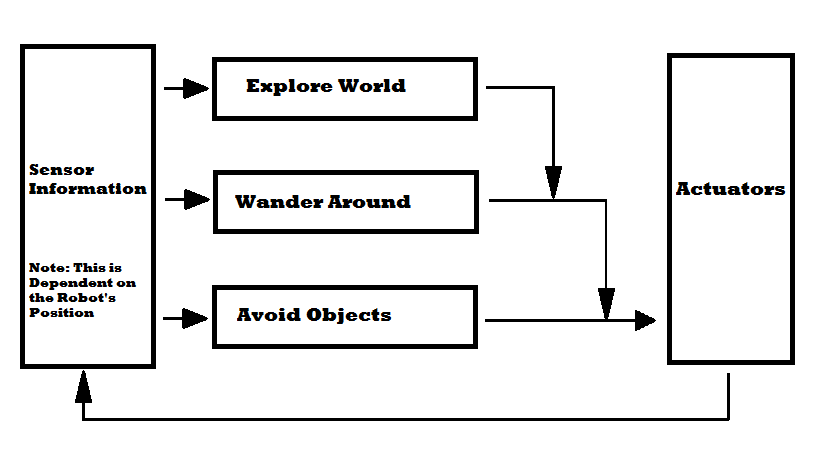
\includegraphics[width = .6\textwidth]{Subsumption_Architecture_Abstract_Diagram.png}
    \caption{Example of a Subsumption architecture \cite{Brooks1999}}
    \label{Subsumption}
\end{figure}

\subsubsection{Deliberative agent architectures}

Compared to a reactive agent, deliberative agents have a more complex structure and are closer to a
human-like, rational behaviour. A deliberative agent is defined as one that
possesses an explicitly represented, symbolic model of the world, and in which
decisions are made via symbolic reasoning \cite{Wooldridge1996}. In other words,
the agent maintains its internal representation of the external environment and
thus is capable to plan its actions, while being in an explicit mental state which
can dynamically change. The Beliefs, Desires and Intentions (BDI) architecture
is the most widely known modelling approach of deliberative agents.

\textbf{BDI architecture}\newline
The BDI paradigm has been used in various applications, such as simulating impacts of climate
change on agricultural land use and production \cite{Caillou2017} or to improve internet
network resilience by creating BDI agents that combats DDoS attacks \cite{Nunes2017}. The main
idea behind this architecture is the emphasis on practical reasoning - the process of figuring
out what to do. There are three logic components that characterize an agent:

\term{Beliefs}
The internal knowledge about the surrounding environment, which
is being constantly updated by agent's perception.

\term{Desires}
What the agent wants to accomplish. An agent can have multiple desires, which can be
hierarchically structured or have different priority.

\term{Intentions}
Intentions are formed when an agent commits to a plan in order to achieve a chosen goal.
The plans are pre-defined within an agent, formally called a \emph{plan library}.
The plan that an agent has set to carry out can dynamically change based on updated beliefs or
desires.

These components together define an agent's \emph{reasoning engine} (fig. (\ref{bdi-schematic})),
which drives the agent's (deliberative) behaviour. 

\begin{figure}[htbp]
    \centering
    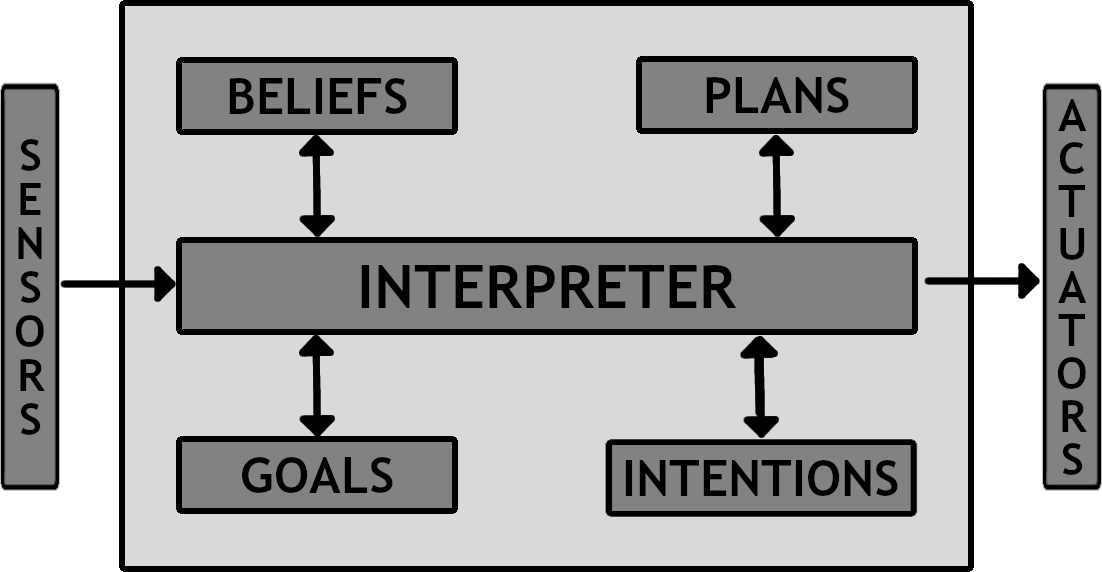
\includegraphics[width = .8\textwidth]{bdi-infographic.png}
    \caption{The BDI architecture schematic}
    \label{bdi-schematic}
\end{figure}

This definition can be made clearer with a simple example scenario - a waiter in a restaurant.
The waiter's \emph{beliefs} are the tables with customers and information about state of each
table (i.e.  choosing menu, waiting for meal, willing to pay etc.). The waiter's \emph{desires}
are to serve customers, for example accept order from a customer. The waiter carries out his
desires by making a plan of \emph{intentions} (e.g. go to table and ask if the customer wants a
drink).

This architecture has its advantage in the fact that the functional decomposition of the system
is clear and intuitive. However, with this architecture, there is a commitment-reconsideration
tradeoff that needs to be optimized \cite{Wooldridge1999}. With too much commitment, there is a
risk of agent overcommitment, where an agent might be trying to achieve a goal that is not
longer valid. On the other hand, if an agent reconsiders too often, there is a risk that the
agent will not achieve any goal because it will switch between intentions too quickly.

\subsubsection{Hybrid approaches}\label{hybrid-arch}

Hybrid architectures try to utilize the best of both worlds of agent modelling. Purely reactive 
agents might lack the ability to solve complex tasks, whereas deliberative architectures are 
challenging to successfully implement on a concrete problem \cite{Anthony2014}. Pre-compiling a plan
library for every possible scenario that can happen in environment with vast amount of complexities
is simply not feasible, due to uncertainties of following effects when agents 
affect the environment. 

The underlying concept of hybrid architectures is to structure agent functionalities into layers 
that interact with each other. This provides several advantages, namely \emph{modularization},
which decomposes the agent's functionalities into distinct modules that have determined 
interfaces. This helps to deal with design complexity. Furthermore, having distinct layers enables 
them to run in parallel, thus increasing an agent's computational ability as well as reactivity
\cite{Mueller1999}.

Generally, amongst the most widely used hybrid architectures, a \emph{controller} layer can be
found, which handles reactive tasks therefore is also connected to the sensor readings, and is 
hierarchically on the lowest level. Then, there are \emph{planning} layers that handle the
logic-based, deliberative tasks and often interact with the controller layer. In-between them, 
there is usually a \emph{sequencing} layer that can suppress output from the reactive layer. 
An example of a well-known hybrid architecture is the \textsubscript{3}T architecture, whose 
abstract model can be seen on the figure (\ref{3-arch}) below.

\begin{figure}[htbp]
    \centering
    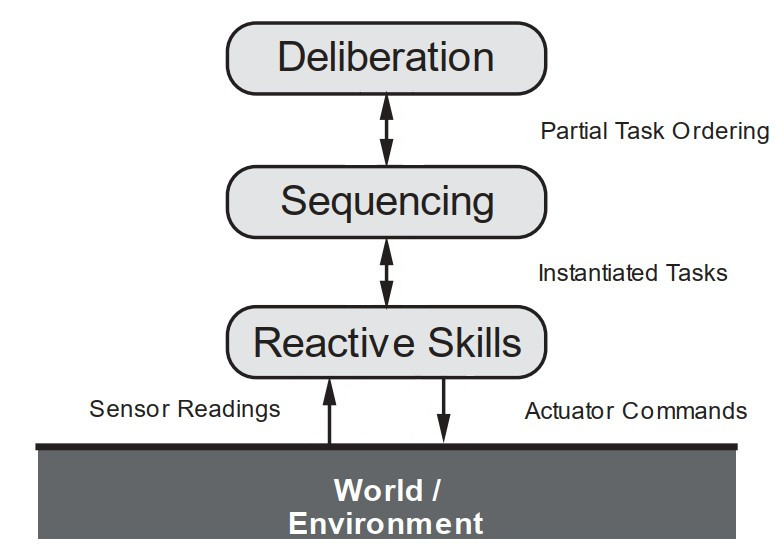
\includegraphics[width=.6\textwidth]{3t-arch.jpg}
    \caption{An architecture model of a \textsubscript{3}T hybrid architecture \cite{Bonasso1995}}
    \label{3-arch}
\end{figure}

\textbf{\textsubscript{3}T architecture}\newline
This architecture builds upon a predecessor architecture called Reactive Action Packages (RAPs)
\cite{Firby1987}. A RAP is essentially a process or a description of how to complete a task using
discrete steps. Note that it has got no planning abilities, i.e. its actions are only based on
current perceived environment state and not on an anticipated state. When a RAP is executed, it
should finish only when it satisfied its outcome or else it will produce a failure state. This
ensures that the agent can self-diagnose a failure and implement some fail-safe mechanisms.
Individual RAPs are queued by the interpreter, in the case of the \textsubscript{3}T architecture it
is called a \emph{sequencer}, which is the intermediate layer between the \emph{reactive skills} and 
\emph{deliberation} layer.

The skills layer is a collection of so-called \emph{skills}. Skills provide an interface of an agent 
to its environment. They are its abilities that allow the agent to transform or maintain a particular 
state in the environment. Each skill has got an expected input and output, which allows to route them 
together. 

Finally, the deliberation layer is responsible for planning on a high level of abstraction, in 
order to make its problem space small. Routine sequences of tasks should not be specified or 
dealt with at this layer. 

\subsubsection{Conclusion}

The different architecture types that were presented can each have a different application where 
they excel. It is also important to note that a line between reactive and deliberative agents 
is not necessarily strict, hence the existence of hybrid architecture types. 

Choosing the optimal agent architecture will depend on the scope of agent goals, 
environment and action space definition. With respect to the topic of this thesis, which is to 
create a framework for implementing various ITS, there isn't a clear-cut choice regarding 
architecture selection. Although the vast majority of ITS share the same goals (see section \ref{its}), 
the operating environment, underlying concepts and also used technology vary substantially.

To put things into a perspective, let's consider ITS introduced in section \ref{its}. 
Systems such as autonomous driving algorithms require high resilience, determinism, 
and high performance, all in extremely dynamic conditions. This would suggest to use a
\emph{reactive} architecture. On the other hand, there are systems such as traffic network management, 
where highly complex problems with lots of variables are considered. Such non-linear behaviour 
requires complex logic and frequent re-planning, therefore more suited for \emph{deliberative}
architectures. Furthermore, when considering the aforementioned cooperative ITS, where the emphasis 
on information sharing and environment awareness is given, it becomes clear that \emph{hybrid} 
architectures which offer both planning and reactive behaviour would be the optimal choice.

As such, when creating the framework for ITS implementation later in this thesis, the
\textsubscript{3}T architecture with RAP utilization will be used.  

\subsection{Interaction between agents}\label{mas-interaction}

It is safe to say that an agent-based ITS system will require some form of agent interaction and
thus communication between individual agents. Interacting agents are able to interact with
other agents within the environment. This concept extends an agent with an interface dedicated
to communication, which makes them able to directly communicate and thus cooperate in a
decentralized fashion.  The concept of cooperation between agents is important in the ITS
modelling context, as these systems facilitate sharing information in-between drivers and also
from the road traffic environment to drivers. Therefore, interaction is a strong component when
considering modelling ITS and road traffic in general. However, this interface also adds to the
system's complexity.

It is expected that most agents would achieve their common goal through cooperation, where some
form of forced altruism is given to the agents. With that being said there could also be
situations where conflicts of interest between agents occur with no clear positive outcome,
i.e. zero-sum games.

One should adhere to some communication principles to facilitate cooperation between agents. As
such, agents should communicate according to Gricean maxims (see the table below)
\cite{Shoham}. This way, the communication and performance overhead is minimized and system 
is more stable. 


\begin{table}[htbp]
    \renewcommand{\arraystretch}{1.7}
    \setlength{\tabcolsep}{1em}
    \caption{Gricean maxims}
    \centering\begin{tabular}{>{\itshape}rl}
       \toprule
       Quantity & Say not more nor less than it is required \\ 
       \midrule
       Relevance &  Stay relevant to the topic of discussion \\
       \midrule
       Manner & Avoid obscurity and ambiguity \\ 
       \midrule
       Quality & Do not give false or unsupported information \\
       \bottomrule
    \end{tabular}
    \label{maxims}
\end{table}

It needs to be said that the agents developed for an ITS system will most likely not be competing 
amongst each other, as the agent reward should be higher the more the agents cooperate. For example, 
when designing cooperative intersections system, the reward function for the individual intersections
(i.e. agents) should take into account not only the throughput on their own intersection but also 
throughput of the whole system. However, that doesn't eliminate the need to negotiate. Consider a 
situation where there are multiple traffic light intersections, each deciding on which phases to 
enable based on the incoming traffic intensity. An optimal option that minimizes cost (e.g. 
travel time) for one agent could have a significant negative effect on other intersections. 
Therefore it is important to achieve an equilibrium that minimizes the overall cost. 

\subsubsection{Organizational decomposition}\label{sec-conflicts}

Before defining the communication protocol, which is arguably the most important aspect of agent 
interaction, it is important to think about the the overall system topology and inter-agent 
relationships. There are two possibilities when designing agent structure.

\textbf{Hierarchical organization}\newline
In hierarchical organization \cite{Damba2007}, agents are organized in a tree structure,
where each level has got a different level of autonomy. The flow of control is 
from top to bottom, i.e. agents in lower level of hierarchy conform to decisions 
from higher levels. 

A simple form of hierarchical organization ensures that there is a low number of conflicts and
the system can be operating by relatively simpler sequential processes where the control flow
is straightforward, however, this also decreases the robustness of the system, because the
control and autonomy not as distributed, e.g. when a failure of a single agent with at a high
hierarchical level causes the whole system to fail. A subtype of this organization - a 
uniform hierarchy, the authority is more distributed among the agents. This makes the
system more fault tolerant and perform graceful degradation in scenarios where one ore more
parts of the system fail \cite{ParasumannaGokulan2010}. Here, a special attention needs to be
given to conflict resolution, which is not always as straightforward, as mentioned earlier. 

\begin{figure}[htbp]
    \centering
    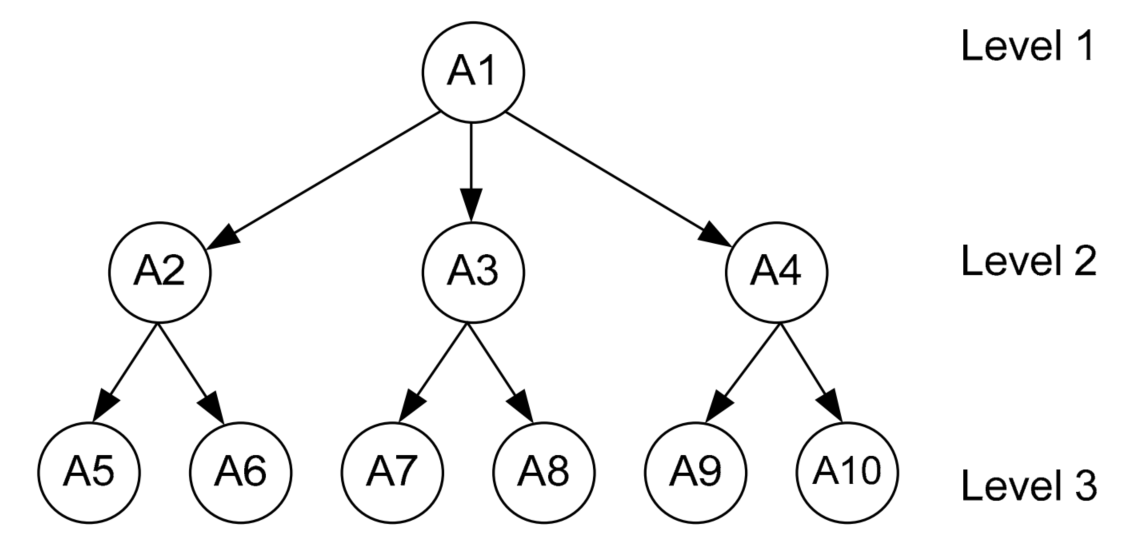
\includegraphics[width=.6\textwidth]{hierarchy.png}
    \caption{Hierarchical agent structure schematic \cite{ParasumannaGokulan2010}}
    \label{hierarchy}
\end{figure}

\textbf{Coalitions}\newline
Another useful agent organization is to organize agents into coalitions. In coalitions, a group of
agents come together for a short time to increase the utility or performance of the individual
agents in a group \cite{ParasumannaGokulan2010}. After the goal is reached or the coalition no 
longer becomes feasible, the coalition ceases to exist. The coalition can have a flat hierarchy, 
with the possibility to have one agent as the leader role for interactions outside the coalition. 
The use of coalitions allows for a highly dynamic system, which on the other hand increases the
system's complexity. 

There are more concepts for structuring a multi-agent system from organizational point of view, 
such as \emph{teams} and \emph{holons}. However, the two mentioned approaches are the most well-suited for 
an ITS system development, as they have been used in more works for this purpose already 
(e.g. \cite{Balaji2007} and \cite{Vijsel2004}). 

In conclusion, the usage of the aforementioned organization should ensure that the system complexity 
is kept as low as possible and the topology is transparent and uncluttered. The hierarchical 
organization can be beneficial when applied to ITS systems such as urban traffic management, where 
conflicts of interests need to be resolved by a capable authority. Whereas, the coalition-based 
organization could be applied to create virtual clusters of connected vehicles (platooning) to apply 
C-ITS features, e.g. dynamic navigation or GLOSA.

\subsubsection{Communication between agents}

As has been stated before, agent communication is a crucial component of a multi-agent system. 
Communication makes for inter-agent interaction beyond cues that an agent receives from the environment 
through its sensors, as agents can either exchange or broadcast information which could not be obtainable 
for the agent otherwise. This allows for deeper and more complex decision making and behaviour design - 
agents can act upon the received information or update their beliefs about the world and provide 
distributed problem solving in general. 

\subsubsection{Agent Communication Language}\label{sec-acl}

Any language, including the one used by agents in an arbitrary system, should have defined its syntax and 
semantics to be an effective medium. Effectively, this means that a dedicated communication
interface for each agent should be defined, with a standardized way of expressing information. 
To satisfy these requirements, a language developed specifically for MAS has been created, 
called \emph{Agent Communication Language} (ACL) \cite{IntelligentPhysicalAgents2001}. 
This specification proposes a standard for agent communication. Most importantly, it defines 
so-called \emph{communicative act} (CA) - a special class of actions that correspond to the basic
building blocks of dialogue between agents. A communicative act has a well-defined, declarative
meaning independent of the content of any given act. CAs are modelled on speech act theory.
Pragmatically, CA's are performed by an agent sending a message to another agent, using a
specified message format. For the index of the defined CAs and their classification, see the
table (\ref{cas}).

Using all of the defined message types is not mandatory in order to use the ACL.
However, the standard introduces ACL-compliant agent requirements that need to be fulfilled. The 
agent requirements are in the table (\ref{requirements}). 

Apart from the mentioned communicative acts, the ACL standard also defines message parameters, which
form the structure of a message (table (\ref{message-parameters})). A sample composed message structure can be found 
in figure (\ref{message-structure}).


\begin{figure}[htbp]
    \centering
    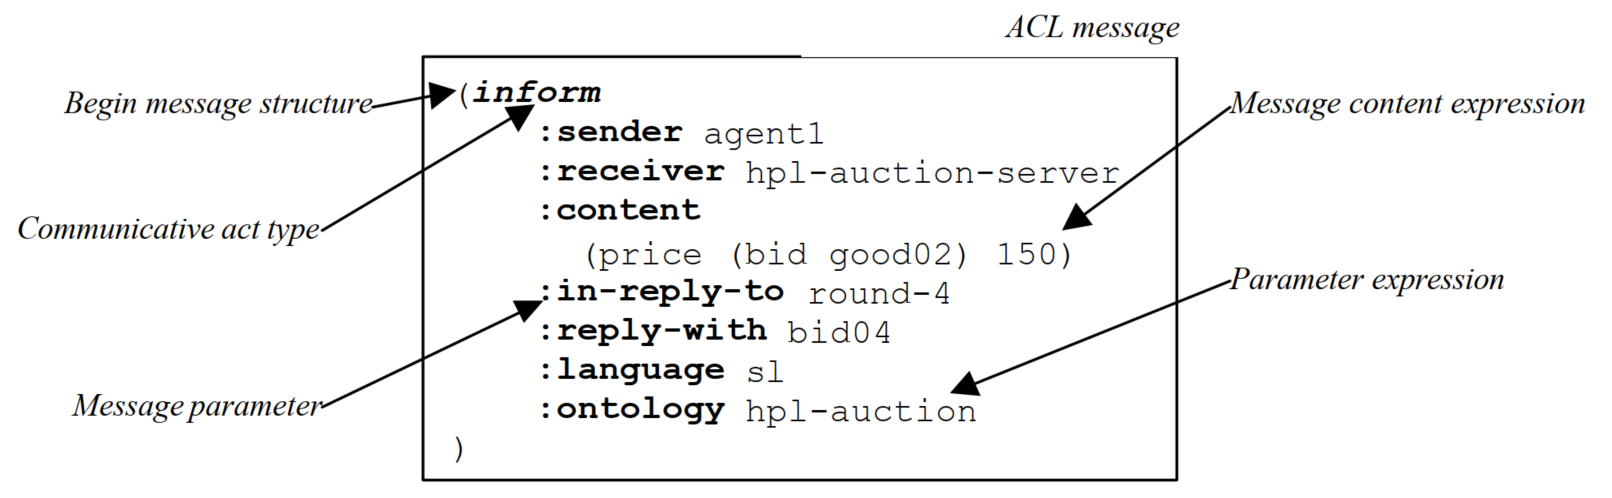
\includegraphics[width=.99\textwidth]{acl-message-structure.png}
    \caption{Main structural components of ACL message \cite{IntelligentPhysicalAgents2001}}
    \label{message-structure}
\end{figure}

It needs to be considered that there are plenty of other standard definitions that are suited for
distributed system interoperability, such as W3C, CORBA, UML and many others, so the choice 
of the ACL needs to be argued. A lot of these applications are based on the so called CRUD set of 
communication primitives - Create, Read, Update and Delete. In contrast to this, ACL defines a lot 
of different communication primitives (i.e. communicative acts). This leads to more complex control 
\cite{Poslad2007}. 
% On a side note, communication between individual units is composed of several layers of communication 
% (e.g. the OSI model). 
% However, The MAS developed in this thesis will be in a closed, virtual space, which 
% will most likely not require integration with other services. This can be further leveraged to our 
% advantage by stripping the language of some redundant message parameters like the \texttt{:transport 
% protocol}, \texttt{:reply-by}, \texttt{:envelope} and other message types, which are not needed
% because communication will be abstracted away and virtualized within the simulation software. 
Also, \cite{Poslad2007} states that The ACL model naturally allows more semantic context
to be included in messages. This can give applications more understandable information about
unexpected events. In addition, the richer set of primitives can lead to more flexible
interaction processes.

\subsubsection{Conclusion}

In this section, the ways how agents interact with each other were described, with respect to the
application scope of this thesis, i.e. applying MAS principles to implement an ITS simulation. The most important
facts are that agent agent organization needs to be considered - despite the fact that MAS are
designed to be highly distributed, giving the agents hierarchical roles can often facilitate
interaction between agents and can decrease system complexity while preserving functionality,
especially during negotiation between agents. Agent grouping should, while also contributing to
decreased system distribution, decrease computation and communication overhead. 

Next, it was found that designing how agents communicate is a crucial part of MAS development
that can get complex, so it is important to keep the ways of sharing information as organized
as possible, which can be done by defining the language, primarily its semantics and associated
syntax.  The cornerstones of inter-agent communication were discussed, and a suitable framework
for the thesis' use-case of setting up communication between agents was investigated and
chosen. The framework of choice was the Agent Communication Language, because its set of
communication primitives already assume the MAS-based use-cases, with predefined requirements,
message parameters and message types while also being open for extension.

Moving forward, the following section will be dedicated to proposing the actual system that will 
be implemented, subject to the topic of the thesis. 

\begin{table}[htbp]
    \renewcommand{\arraystretch}{1.7}
    \footnotesize
    \caption{Categories of communicative acts \cite{IntelligentPhysicalAgents2001}}
    % \setlength\tabcolsep{0pt}
    \centering
    \begin{tabular}{|>{\ttfamily}r| *{4}{>{\centering}c|} >{\centering\arraybackslash}c|}
        \hline
        \hfill \rmfamily\textbf{Communicative act} \hspace*{\fill} & \rot{\textbf{Information passing}} & \rot{\textbf{Requesting information}} & \rot{\textbf{Negotiation}} & \rot{\textbf{Action} performing} & \rot{\textbf{Error} handling} \\
        \hline
        accept-proposal                    &                              &                                 &     $\blacksquare$   &                            &                         \\\hline
        agree                              &                              &                                 &                      &    $\blacksquare$          &                         \\\hline
        cancel                             &                              &                                 &                      &     $\blacksquare$         &                         \\\hline
        cfp                                &                              &                                 &     $\blacksquare$   &                            &                         \\\hline
        confirm                            &    $\blacksquare$            &                                 &                      &                            &                         \\\hline
        disconfirm                         &    $\blacksquare$            &                                 &                      &                            &                         \\\hline
        failure                            &                              &                                 &                      &                            &     $\blacksquare$      \\\hline
        inform                             &   $\blacksquare$             &                                 &                      &                            &                         \\\hline
        inform-if (macro act)               &    $\blacksquare$            &                                 &                      &                            &                         \\\hline
        inform-ref (macro act)              &    $\blacksquare$            &                                 &                      &                            &                         \\\hline
        not-understood                     &                              &                                 &                      &                            &       $\blacksquare$    \\\hline
        propose                            &                              &                                 &    $\blacksquare$    &                            &                         \\\hline
        query-if                           &                              &           $\blacksquare$        &                      &                            &                         \\\hline
        query-ref                          &                              &            $\blacksquare$       &                      &                            &                         \\\hline
        refuse                             &                              &                                 &                      &     $\blacksquare$         &                         \\\hline
        reject-proposal                    &                              &                                 &    $\blacksquare$    &                            &                         \\\hline
        request                            &                              &                                 &                      &    $\blacksquare$          &                         \\\hline
        request-when                       &                              &                                 &                      &     $\blacksquare$         &                         \\\hline
        request-whenever                    &                              &                                 &                      &     $\blacksquare$         &                         \\\hline
        subscribe                          &                              &            $\blacksquare$       &                      &                            &                         \\\hline
    \end{tabular}
    \label{cas}
\end{table}

\begin{table}[htbp]
    \caption{The ACL-compliant agent requirements \cite{IntelligentPhysicalAgents2001}}
    \renewcommand{\arraystretch}{1.7}
    \centering\begin{tabular}{p{.9\textwidth}}
\toprule
\textbf{Requirement 1}:
Agents should send not-understood if they receive a message that they do not recognise or they are unable to
process the content of the message. Agents must be prepared to receive and properly handle a not-understood
\\ \midrule
\textbf{Requirement 2}:
An ACL compliant agent may choose to implement any subset (including all, though this is
unlikely) of the predefined message types and protocols. The implementation of these messages
must be correct with respect to the referenced act's semantic definition.
 \\ \midrule
\textbf{Requirement 3}:
An ACL compliant agent which uses the communicative acts whose names are defined in the specification must
implement them correctly with respect to their definition.
\\ \midrule
\textbf{Requirement 4}:
Agents may use communicative acts with other names, not defined in the specification document,
and are responsible for ensuring that the receiving agent will understand the meaning of the
act. However, agents should not define new acts with a meaning that matches a pre-defined
standard act.
 \\ \midrule
\textbf{Requirement 5}:
An ACL compliant agent must be able to correctly generate a syntactically well formed message in the transport
form that corresponds to the message it wishes to send. Symmetrically, it must be able to translate a character
sequence that is well-formed in the transport syntax to the corresponding message.
\\ \bottomrule
    \end{tabular}
    \label{requirements}
\end{table}

\begin{table}[htbp]
    \footnotesize
    \renewcommand{\arraystretch}{1.8}
    \caption{Pre-defined message parameters \cite{IntelligentPhysicalAgents2001}}
    \centering\begin{tabularx}{.8\textwidth}{>{\ttfamily}rX}
        \toprule
        \multicolumn{1}{p{8em}}{\bf \centering Message \newline Parameter} & \bf \centering Meaning \arraybackslash                \\\midrule
        :sender                                                            & Denotes the identity of the sender of the message,
                                                                            i.e. the name of the agent of the communicative act. \\\midrule
        :receiver                                                          & Denotes the identity of the intended recipient of the
                                                                            message. \\\midrule
        :content                                                           & Denotes the content of the message; equivalently
                                                                            denotes the object of the action. \\\midrule
        :reply-with                                                        & Introduces an expression which will be used by the
                                                                            agent responding to this message to identify the
                                                                            original message. Can be used to follow a
                                                                            conversation thread in a situation where multiple
                                                                            dialogues occur simultaneously. \\\midrule
        :in-reply-to                                                       & Denotes an expression that references an earlier
                                                                            action to which this message is a reply. \\\midrule
        :envelope                                                          & Denotes an expression that provides useful
                                                                            information about the message as seen by the
                                                                            message transport service. \\\midrule
        :language                                                          & Denotes the encoding scheme of the content of the
                                                                            action. \\\midrule
        :ontology                                                          & Denotes the ontology which is used to give a
                                                                            meaning to the symbols in the content expression. \\\midrule
        :reply-by                                                          & Denotes a time and/or date expression which
                                                                            indicates a guideline on the latest time by which the
                                                                            sending agent would like a reply. \\\midrule
        :protocol                                                          & Introduces an identifier which denotes the protocol
                                                                            which the sending agent is employing. \\\midrule
        :conversation-id                                                   & Introduces an expression which is used to identify an
                                                                            ongoing sequence of communicative acts which
                                                                            together form a conversation. \\\bottomrule
    \end{tabularx}
    \label{message-parameters}
\end{table}
\clearpage

\end{document}